\chapter{Experimente und Resultate}
In diesem Kapitel wird der Aufbau der Experimente und die dazugehörigen Resultate erklärt. Wir werden alle Experimente auch mit der Domäne Union durchführen, welche nichts anderes als eine Sammlung aller Domänen ist. Bei der Besprechung der Resultate ist mit alle Domänen, jedoch alle exklusiv Union gemeint. Wir werden Union jeweils als einen Spezialfall behandeln.
Zur Validierung der Resultate verwenden wir ausschliesslich den $F1_{pos,neg}$. Wir entschieden uns dazu, da der $F1_{neu}$ tendenziell immer besser ist als $F1_{pos}$, oder $F1_{neg}$ und auch in den Trainingssets sind positive und negative Beispiele deutlich seltener vertreten. Anhand konkreter Zahlen können wir diese Vermutung bestätigen. Die einzelnen Mittelwerte, bei dem Experiment \ref{sec:Distant-Phase and Word-Embedding} sind wie folgt: $F1_{pos}$ 0.479, $F1_{neg}$ 0.455 und $F1_{neu}$ 0.581. Dies, obwohl die Validierung nur auf die Veränderung des $F1_{pos,neg}$ reagiert und wir die Lernrate bei positiven und negativen Beispiele zusätzlich mit Class-Weights verstärken.
\fixme{Verteilung Pos/Neg/Neut}
\section{Distant-Phase \& Word-Embeddings}\label{sec:Distant-Phase and Word-Embedding}
Ziel dieser Experimente ist es, herauszufinden welche Kombination von Word-Embeddings (siehe Kapitel Daten) und Distant-Phase (siehe Kapitel Daten) die besten Ergebnisse für die jeweilige Domäne liefert. Aufgrund dieser Ergebnisse werden alle nachfolgenden Experimente mit der bestmöglichen Konfiguration durchgeführt.
\subsection{Aufbau Distant-Phase \& Word-Embeddings} Pro Domäne werden 12 Experimente durchgeführt, dies resultiert aus der Kombination mit 3 Word-Embeddings und den 2 Distant-Phases (siehe Kapitel Daten), zusätzlich verwenden wir zufällig initialisierten Word-Embeddings und wir testen auch das weglassen der Distant-Phase. Bei jedem Experiment werden die maximale Anzahl Trainingsdaten der Zieldomäne verwendet und entsprechend auf der gleichen Domäne validiert. So erhalten wir ein CNN, welches auf die Zieldomäne zugeschnitten ist und die bestmögliche Ergebnisse liefert.
\subsection{Resultate Distant-Phase \& Word-Embeddings}
In der Tabelle \ref{tbl:word_embeddings} befinden sich die erzielten $F1_{pos,neg}$ nach dem testen mit der Zieldomäne. Die besten Werte pro Domäne sind jeweils fett markiert.
\paragraph{Die Wahl der Distant-Phase und Word-Embeddings tragen massgeblich zum Resultat bei.} Wie wir erkennen können, variieren die Werte innerhalb einer Domäne recht stark. Der Unterschied vom besten $F1_{pos,neg}$ zum Schlechtesten, beträgt in fast allen Domänen ~15\%. Auch wenn wir nur die Word-Embeddings, oder nur die Distant-Phases miteinander vergleichen, sind die Unterschiede teilweise sehr gross. Somit ist für uns klar ersichtlich, dass die Wahl der besten Konfiguration aus Word-Embeddings und Distant-Phase einen erheblichen Einfluss auf die Resultate hat.
\paragraph{Weshalb liefern Random Word-Embeddings und None Distant-Phase Experimente brauchbare Ergebnisse?} Wir sehen in \ref{tbl:word_embeddings}, dass die zufällige Initialisierung der Word-Embeddings, oder aber das Auslassen einer Distant-Phase, keinen grossen negativen Effekt auf das CNN hat. Wenn man jedoch die letzte Spalte Avg. betrachtet sehen wir, dass die Ergebnisse mit None Distant-Phase pro Word-Embeddings im Schnitt immer schlechter sind. Wichtig hierbei ist auch, dass die Word-Embeddings und die Distant-Phase sich gegenseitig beeinflussen. Das bedeutet, dass während der Distant-Phase schlechte Word-Embeddings mehr profitieren, als von Anfang an gut performierend Word-Embeddings. Andersherum, können gut performierende Word-Embeddings eine fehlende Distant-Phase kompensieren. Aus der Tabelle entnehmen wir, dass bei jeder Domäne, die Kombination aus Random Word-Emebddings und None Distant-Phase, fast immer die schlechtesten Ergebnisse liefert. Die Ausnahmen sind schlechter performierende Word-Embeddings in der Kombination, mit None Distant-Phase.

\begin{figure}[h]
	\centering
	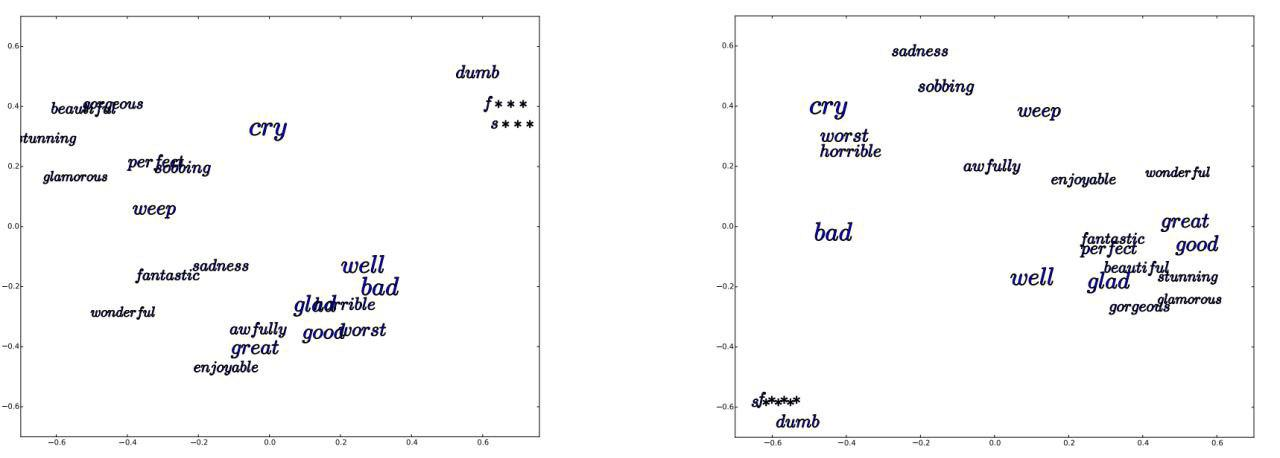
\includegraphics[width=10cm]{img/word_emebddings_veraenderung.jpg}
	\caption{Schematische Darstellung}
	\label{fig:word_embeddings}
\end{figure}
\fixme{Grafik mit unseren Embeddings ersetzen und entsprechend beschriften. und im text dann referenzieren}

\paragraph{Union scheint eine Option zu sein.} Wenn wir in der Tabelle \ref{tbl:word_embeddings} die Zeilen betrachten, sehen wir, dass die einzelnen Werte bis zu 20\% variieren. Vergleichen wir den Durchschnitt einer Zeile mit dem Ergebnis des Union CNN, liegen die Werte immer sehr nahe beieinander und sind meistens sogar besser. Sofern nun ein Sentiment-Classifier für eine noch unbekannte Domäne benötigt wird, für welche wir die beste Konfiguration noch nicht kennen, scheint es eine  Option zu sein mit einem Union CNN zu starten. Wir werden später diesen Theorie noch genauer prüfen, indem wir mit einer unbekannten Domäne, ein Union CNN testen. Zusätzlich werden wir versuchen herauszufinden, ob gewisse Domänen verträglicher miteinander sind, als Andere. Zum jetzigen Zeitpunkt können wir aber die folgende Aussage treffen: Anstelle eines zufälliges CNN mit einer zufälligen Domäne zu verwenden, um eine neue, unbekannte Domäne zu testen, scheint es ratsamer zu sein ein Union CNN zu verwenden. Wir verlieren dadurch vielleicht ein paar Prozentpunkte beim $F1_{pos,neg}$, entfernen jedoch die zum Teil recht grosse Streuung des $F1_{pos,neg}$.
\begin{table*}[]

	\small
	\centering
	
	\begin{adjustbox}{max width=\textwidth}
		
		\begin{tabular}{l|l|l|l|l|l|l|l|l|l|l||l|}
			& Dist. Phase 
			&  \specialcell{DAI \\\textit{(T/ 3.2k)}}
			&  \specialcell{MPQ \\\textit{(N/ 8.8k)}}
			&  \specialcell{DIL \\\textit{(R/ 3.4k)}}
			&  \specialcell{TAC \\\textit{(R/ 2.1k)}}
			&  \specialcell{SEM \\\textit{(H/ 3.1k)}}
			&  \specialcell{JCR \\\textit{(Q/ 1k)}}
			&  \specialcell{SEval \\\textit{(T/ 8.2k)}}
			&  \specialcell{HUL \\\textit{(R/ 3.1k)}}
			&  Union
			&  Avg.  \\
			\hline
			\multirow{3}{*}{Random}
			& None 		& 0.599 		& 0.469 		& 0.509 		& 0.577 					& 0.436 		& 0.263 		& 0.598 		& 0.513 		& 0.550& 0.502\\
			& Reviews	& \textit{0.698}& \textit{0.539}& \textit{0.595}& \textbf{\textit{0.714}} 	& \textit{0.477}& \textit{0.401}& \textit{0.659}& \textit{0.659}& \textit{0.603}& 0.594\\
			& Twitter 	& 0.684 		& 0.490 		& 0.523 		& 0.612 					& 0.468 		& 0.399 		& 0.659 		& 0.517 		& 0.595&0.550\\
			\hline
			\multirow{3}{*}{News}
			& None 		&  0.631 			& \textbf{\textit{0.581}}& 0.485 		 & 0.644 		  & 0.527 		   & 0.405 			& 0.673 				& 0.480 		 & 0.615&0.560\\
			& Reviews 	&  0.692 & 0.563 				 & 0.590 & 0.682 & 0.519 		   & 0.433 & 0.685 		& 0.649 & \textbf{\textit{0.624}}& 0.604\\
			& Twitter 	&  0.678 			& 0.567 				 & 0.546 		 & 0.676 		  & 0.539 & 0.412 			& \textbf{\textit{0.691}}& 0.554 		 & 0.444&0.568 \\
			\hline
			\multirow{3}{*}{Twitter} 
			& None 		&  0.629 & 0.504 & 0.507 & 0.585 & 0.541 & 0.360 & 0.629 & 0.511 & 0.584& 0.539\\
			& Reviews 	&  0.701 & \textit{0.540} & \textbf{\textit{0.603}} & \textit{0.694} & 0.472 & 0.383 & 0.683 & \textit{0.657} & \textit{0.611}& 0.594\\
			& Twitter 	&  \textbf{\textit{0.734}} & 0.518 & 0.543 & 0.652 & \textbf{\textit{0.554}} & \textit{0.412} & \textit{0.685} & 0.553 & 0.610&0.585 \\
			\hline
			\multirow{3}{*}{Wikipedia}
			& None 		&  0.553 & 0.529 & 0.455 & 0.570 & \textit{0.506} & 0.375 & 0.613 & 0.451 & 0.567&0.513 \\
			& Reviews	&  0.661 & 0.542 & \textit{0.569} & \textit{0.684} & 0.500 & \textbf{\textit{0.457}} & 0.622 & \textbf{\textit{0.666}} & 0.577& 0.586\\
			& Twitter 	&  \textit{0.663} & \textit{0.544} & 0.520 & 0.619 & 0.505 & 0.411 & \textit{0.642} & 0.531 & \textit{0.580}&0.557 \\
			\hline
			\hline
			Full Average    & - & 0.660 & 0.532 & 0.537 & 0.643 & 0.504 & 0.393 & 0.653 & 0.562 & 0.580 & -\\
			\hline
			Rand. Avg. & - & 0.660& 0.499&	0.542 & 0.635 & 0.460 & 0.354 & 0.639 &	0.563&	0.583 & 0.548\\
			News Avg.  & - & 0.667& \textbf{\textit{0.570}} & 0.540& \textbf{\textit{0.668}} & \textbf{\textit{0.528}} & \textbf{\textit{0.417}} & \textbf{\textit{0.683}} & 0.561 & 0.561 & 0.577\\
			Twit. Avg. & - & \textbf{\textit{0.688}} & 0.521& \textbf{\textit{0.551}} & 0.643& 0.522 & 0.385& 0.666& \textbf{\textit{0.573}} & \textbf{\textit{0.602}} & 0.572\\
			Wiki. Avg  & - & 0.626& 0.538&	0.515&	0.625&	0.504&	0.414&	0.626&	0.549&	0.575&	0.552\\
			\hline
			- & None Avg. & 0.603&	0.520&	0.489&	0.594&	0.502&	0.351&	0.628&	0.489&	0.579&	0.528\\
			- & Rev. Avg. & 0.688&	\textbf{\textit{0.546}}&	\textbf{\textit{0.589}}&	\textbf{\textit{0.694}}&	0.492&	\textbf{\textit{0.418}}&	0.662&	\textbf{\textit{0.658}}&	\textbf{\textit{0.604}}&	0.595\\
			-  & Twi. Avg. & \textbf{\textit{0.690}}&	0.530&	0.533&	0.640&	\textbf{\textit{0.517}}&	0.409&	\textbf{\textit{0.669}}&	0.539&	0.558&	0.565\\
			\hline
		\end{tabular}
	\end{adjustbox}
	\caption{\textit{F1 Score aller Kombinationen aus Word-Embeddings und Distant-Phase pro Domäne. Die letzte Spalte ist der Durchschnittswert der jeweiligen Zeile und somit Domänen übergreifend Die unteren 8 Zeilen sind jeweils die Durchschnittswerte, entsprechend der Beschriftung, pro Domäne. Die Texttypen der Domäne sind folgendermassen codiert: T: Tweets, N: News, R: Reviews, H: Headlines and Q: Quotations.}}
	\label{tbl:word_embeddings}
\end{table*}

\section{Crossdomain}
Mit dieser Experimentreihe möchten wir herausfinden, wie gut die besten CNN \ref{sec:Distant-Phase and Word-Embedding} auf einer fremden Domäne performen. Wir möchten dabei auch untersuchen, ob es Domänen gibt welche sich mehr eignen zu kombinieren, als Andere.
\subsection{Aufbau Crossdomain} Wir trainieren ein CNN für eine Fremddomäne und validieren während dem Training auch auf derselbigen. Anschliessend testen wir den Sentiment Classifier auf den anderen Domänen, welche in diesem Experiment die Zieldomäne ist, einzeln. Wir verwenden jeweils alle zur Verfügung stehenden Trainings- und Testdaten.
Man könnte sich auch überlegen, anstelle der besten Konfiguration für die Fremddomäne, die beste Konfiguration für die Zieldomäne zu wählen. Wir entschieden dafür, weil während dem Training auch die Embeddings angepasst werden und in einem Anwendungsfall die beste Konfiguration der Zieldomäne noch unbekannt ist.

\subsection{Resultate Crossdomain}\label{subsec:Resultate Crossdomain}
In der Tabelle \ref{tbl:ablation} befinden sich die erzielten $F1_{pos,neg}$ nach dem testen mit der Zieldomäne. Die besten Werte pro Domäne sind jeweils fett markiert.
\begin{table*}[!t]
	\centering
	\small
	
	\begin{tabular}{l|lllllllll|ll}
		\backslashbox{Train}{Test}
		&  \specialcell{DAI \\\textit{T}}
		&  \specialcell{MPQ \\\textit{N}}
		&  \specialcell{DIL \\\textit{R}}
		&  \specialcell{TAC \\\textit{R}}
		&  \specialcell{SEM \\\textit{H}}
		&  \specialcell{JCR \\\textit{Q}}
		&  \specialcell{SEval \\\textit{T}}
		&  \specialcell{HUL \\\textit{R}}	& Union \\
		
		\hline
		DAI T	&\textbf{0.734}	&0.161	&0.401	&0.369	&0.283	&0.269	&0.554	&0.397	&0.447 \\
		MPQ N 	&0.495	&\textbf{0.581}	&0.307	&0.402	&0.313	&0.411	&0.471	&0.318	&0.489 \\
		DIL R	&0.381	&0.210	&\textbf{0.603}	&0.478	&0.135	&0.227	&0.365	&0.602	&0.350 \\
		TAC R	&0.395	&0.376	&0.501	&\textbf{0.714}	&0.360	&0.409	&0.480	&0.517	&0.442 \\
		SEM H	&0.360	&0.148	&0.188	&0.247	&\textbf{0.554}	&0.054	&0.250	&0.181	&0.227 \\
		JCR Q	&0.450	&0.319	&0.402	&0.461	&0.254	&\textbf{0.457}	&0.402	&0.452	&0.384 \\
		SEval T	&0.525	&0.441	&0.489	&0.577	&0.445	&0.421	&\textbf{0.691}	&0.479	&0.578 \\
		HUL R	&0.404	&0.252	&0.567	&0.535	&0.176	&0.312	&0.392	&\textbf{0.666}	&0.373 \\
		\hline
		Union 	&\textbf{0.725}	&0.55	&0.554	&0.614	&0.422	&0.465	&0.69	&0.528	&0.624 \\
		\hline
		\hline
		FD Avg. &0.43	&0.272	&0.408	&0.438	&0.281	&0.301	&0.416	&0.421	&0.411 \\
		Diff.	&0.304	&0.308	&0.195	&0.276	&0.273	&0.156	&0.275	&0.245	&0.213 \\
		
	\end{tabular}
	\caption{\textit{Results obtained by training on TD and evaluation on all domains. The line \emph{FD Avg.} shows the average scores for each TD when trained on a FD. The line \emph{Diff.} shows the difference between the best score of TD and FD Avg.}}
	\label{tbl:cross-domain}
\end{table*}
\paragraph{Die besten Resultate erhalten wir auf der eigenen Domäne.} Wie erwartet erhalten wir das beste Ergebnis wenn wir auf der gleichen Domäne validieren und testen. Die Varianz in den Ergebnissen ist enorm hoch. Es scheint so, dass es strukturell grosse Unterschiede zwischen den verschiedenen Domänen gibt. Wir möchten herausfinden, welche Strukturen relevant sind, um Domänen zusammenfassen zu können.
Bei der Zeile Union fällt sofort auf, dass es diese hohe Varianz nicht gibt. Dies scheint unsere Vermutung in \ref{subsec:Resultate Crossdomain} zu bestätigen, dass wir bei einer neuen, unbekannten Domäne die zuverlässigeren Ergebnisse erhalten, wenn wir ein Union CNN benutzen, anstelle eines zufälligen für eine andere Domäne spezialisiertes CNN.
\paragraph{Ausprägung des Sentiment} Es gibt zwei Aspekte die wir uns in diesem Zusammenhang überlegen. Das Eine ist die Ausprägung des Sentiment, also wie stark positiv/negativ ein Text verfasst wird. Die zweite Überlegung, wie konzentriert liegt der Sentiment vor. Bei Tweets, wie auch bei Reviews vermuten wir, dass die Ausprägung des Sentiment stärker ist. Eine Privatperson schreibt sehr deutlich, wenn ihr etwas nicht passt, oder aber gefällt. Dies im Gegensatz zu News Meldungen, Headlines und Quotations, bei welchen eine gewisse Professionalität verlangt wird und somit die Ausprägung des Sentiments weniger stark ist.
\fixme{Domänenname: Beispiel \emph{HUL-reviews}}
Tweets haben zusätzlich den Vorteil, dass die Konzentration des Sentiments sehr hoch ist. Es wird oft mit wenigen Wörtern, eine klar positiv/negativ Meldung verfasst.
\fixme{Konzentration mehr umschreiben}
\fixme{Wortstatistik}
\paragraph{Ein Union CNN ist nie besser als für die Zieldomäne trainiertes CNN.}
\paragraph{Korreliert die Varianz mit der Datenmenge} In der Tabelle \ref{tbl:varianz} sehen wir die Varianz, Standartabweichung, Anzahl Trainingsdaten und den durchschnittlich erzielten $F1_{pos,neg}$ nach dem Testen mit allen anderen Domänen pro CNN. Wir möchten untersuchen, ob eine Korrelation zwischen diesen Grössen besteht.

\begin{table}[!t]
	\centering
	\small
	\begin{tabular}{l|cccc}
		&\specialcell{Varianz}&\specialcell{Standart-\\abweichung}    &\specialcell{Trainings-\\daten}  & \specialcell{Avg \\$F1_{pos,neg}$}\\
		\hline
		DAI &0.028&	0.159&	3.2k	&0.402\\
		MPQ	&0.009&	0.091&	8.8k  	&0.421\\
		DIL	&0.028&	0.157&	3.4k  	&0.372\\
		TAC	&0.012&	0.102&	2.1k  	&0.466\\
		SEM	&0.020&	0.134&	3.1k  	&0.246\\
		JCR	&0.005&	0.067&	1k 		&0.398\\
		SEval&0.007&0.082&	8.2k  	&0.516\\
		HUL	&0.025&	0.148&	3.1k 	&0.408\\
		Union &0.012&0.102&	32.9k	&0.553
		
	\end{tabular}
	\caption{\textit{Varianz, Standartabweichung, Anzahl Trainingsdaten und Avg $F1_{pos,neg}$ pro CNN.}}
	\label{tbl:varianz}
\end{table}
\paragraph{Fast 20\% Differenz von der besten zu schlechtesten Domäne.} Hängt es mit der Datenmenge, oder Domäne zusammen....
Erklärung, zum Beispiel Twitter einfache Domäne klar positiv/negativ, bei news texten z.B weniger
\paragraph{Gibt es so etwas wie Domänenfreundlich?} Differenz von fast 20\% sind auch im FD Avg ersichtlich...., Streuung zum Teil sehr gross 0.188 bis 0.567; 0.054 bis 0.054 (SEM/JCR wenig Daten??)

\section{Ablation}
\subsection{Aufbau Ablation}
\subsection{Resultate Ablation}
\begin{table}[!t]
	\centering
	\small
	\begin{tabular}{l|ccc}
		&\specialcell{Ablation Sys. \\ without TD}&\specialcell{Specific TD\\System}    &Diff.  \\
		\hline
		DAI 	&0.658&	0.734&	0.076  \\
		MPQ	&0.404&	0.581&	0.177  \\
		DIL	&0.573&	0.603&	0.030  \\
		TAC	&0.558&	0.714&	0.156  \\
		SEM	&0.426&	0.554&	0.128  \\
		JCR	&0.485&	0.457&	-0.029 \\
		SEval	&0.658&	0.691&	0.033  \\
		HUL	&0.566&	0.666&	0.099
		
	\end{tabular}
	\caption{\textit{Results of the ablation experiments.}}
	\label{tbl:ablation}
\end{table}
\paragraph{Ist die Wahl einer Domänen statistisch Signifikant bezüglich dem $F1_{pos,neg}$?} Wir sehen in der Tabelle \ref{tbl:cross-domain}, dass die Ergebnisse doch sehr stark variieren und möchten mit einer zweifaktoriellen Varianzanalyse untersuchen, ob die abhängige Variable $F1_{pos,neg}$ von den unabhängigen Variablen Zieldomäne und Fremddomäne abhängig ist.
Als Signifikanzniveau wählen wir 0.05. Das Ergebnis dieser Analyse sehen wir in der Tabelle \ref{tbl:ANOVA}. Wir sehen auf den ersten Blick, dass der P-Wert bei beiden unabhängigen Variablen unter unserem Signifikanzniveau von 0.05 liegen. Das bedeutet beide unabhängigen Variablen sind statistisch gesehen signifikant und somit ist es relevant mit welcher Domäne wir ein CNN trainieren. Der P-Wert und die Prüfgrösse F zeigen uns, dass das Ergebnis stärker durch die Fremddomäne beeinflusst wird, als die Zieldomäne. Dass der Resultierende $F1_{pos,neg}$ stärker von den Trainingsdaten abhängt, als der Zieldomäne mit der wir den Sentiment-Classifier testen, erstaunt uns nicht.
Trotzdem wollten wir diesen Sachverhalt Statistisch untersuchen, um herauszufinden, wo die Optimierungspotenziale liegen und ob es Unterschiede zwischen den einzelnen Domänen gibt.
\fixme{P-wert und F-Wert und 0.05 kurz Erklärung}
\begin{table}[!t]
	\begin{adjustbox}{max width=\textwidth}
	\centering
	\small
	\begin{tabular}{c|cccccc}
		\specialcell{Streuungsursache}&\specialcell{Quadratsummen}    &\specialcell{Freiheitsgrade}  & \specialcell{Mittlere Quadratsumme}	& \specialcell{Prüfgrösse (F)}	& \specialcell{P-Wert} & \specialcell{Kritischer F-Wert}\\
		\hline
		Zieldomäne 		&0.357	&8		&0.045	&3.516	&0.00199	&2.087\\
		Fremddomäne		&0.566	&8		&0.071 	&5.577	&0.00002	&2.087\\
		Zufallsfehler	&0.811	&64		&-  	&-		&-			&-\\
		Summe			&0.012	&80		&-  	&-		&-			&-
	\end{tabular}
	\end{adjustbox}
	\caption{\textit{Zweifaktorielle Varianzanalyse mit Signifikanzniveau 0.05}}
	\label{tbl:ANOVA}
\end{table}











